\documentclass[a4paper,12pt]{article}

\usepackage[utf8]{inputenc}
\usepackage[T1]{fontenc}
\usepackage[brazil]{babel}
\usepackage{amsmath}
\usepackage{amssymb}
\usepackage{graphicx}
\usepackage{float}
\usepackage{geometry}
\usepackage{listings}
\usepackage{xcolor}
\usepackage{hyperref}
\usepackage{booktabs}
\usepackage{array}
\usepackage{caption}
\usepackage[numbers]{natbib}
\usepackage{subcaption}

\geometry{margin=2.5cm}

\hypersetup{
    colorlinks=true,
    linkcolor=blue!60!black,
    citecolor=blue!60!black,
    urlcolor=blue!60!black
}

\definecolor{codebg}{rgb}{0.97,0.97,0.97}
\definecolor{codeframe}{rgb}{0.8,0.8,0.8}
\definecolor{keyword}{rgb}{0.0,0.0,0.7}
\definecolor{comment}{rgb}{0.4,0.4,0.4}
\definecolor{string}{rgb}{0.2,0.5,0.2}

\lstdefinelanguage{VHDL2}{
    morekeywords={library, use, entity, architecture, port, in, out, std_logic,
                  std_logic_vector, signal, begin, end, process, if, then, else,
                  elsif, when, others, downto, and, or, not, xor, nor,
                  std_ulogic, all, is, case, map, component},
    sensitive=false,
    morecomment=[l]{--},
    morestring=[b]"
}

\lstset{
    language=VHDL2,
    backgroundcolor=\color{codebg},
    frame=single,
    rulecolor=\color{codeframe},
    basicstyle=\ttfamily\small,
    keywordstyle=\color{keyword}\bfseries,
    commentstyle=\color{comment}\itshape,
    stringstyle=\color{string},
    numbers=left,
    numberstyle=\tiny\color{gray},
    numbersep=8pt,
    breaklines=true,
    captionpos=b,
    tabsize=4
}

\title{
    \large Centro Universitário Dom Helder --- Departamento de Ciência da Computação \\[0.4cm]
    \rule{\linewidth}{0.5pt} \\[0.3cm]
    \textbf{Implementação de Detecção de Overflow em uma Unidade Aritmética MIPS de 4 \textit{bits}} \\[0.2cm]
    \rule{\linewidth}{0.5pt}
}
\author{Enzo Rocha Leite Diniz Ribas}
\date{\today}

\begin{document}

\maketitle

\begin{abstract}
Este trabalho apresenta a implementação do mecanismo de detecção de overflow em uma
Unidade Lógica e Aritmética (ULA) baseada na arquitetura MIPS. A ULA desenvolvida
suporta as operações lógicas AND, OR e NOR, além das operações aritméticas ADD e SUB
e da operação de comparação SLT (\textit{Set Less Than}). O principal objetivo foi
implementar e validar a lógica responsável por identificar situações de overflow
durante operações aritméticas com números representados em complemento de dois. Os
resultados obtidos confirmam a correta detecção de overflow nos casos esperados,
sem geração de falsos positivos em operações lógicas.
\end{abstract}

\newpage
\tableofcontents
\newpage

\section{Introdução}

A Unidade Lógica e Aritmética (ULA) é um dos componentes centrais de qualquer
processador moderno, sendo responsável pela execução de operações matemáticas e
lógicas sobre dados binários. Na arquitetura MIPS32 (\textit{Microprocessor without
Interlocked Pipeline Stages}), a ULA desempenha papel fundamental na execução de
instruções do tipo R e em diversas operações realizadas ao longo do ciclo de
execução de uma instrução.

Durante operações aritméticas com números inteiros com sinal, pode ocorrer uma
condição denominada transbordamento ou \textit{overflow}, que consiste em o resultado da operação exceder a faixa de
representação disponível para o número de bits utilizado. Em um sistema de 32 bits
com complemento de dois, essa faixa é $[-2^{31},\, 2^{31}-1]$. A não detecção de overflow compromete a integridade
dos resultados e pode levar a comportamentos incorretos do programa.

Este trabalho descreve a implementação e validação de uma ULA de 4 bits compatível
com a arquitetura MIPS estudada na disciplina de Arquitetura e Organização de Computadores, incluindo o mecanismo de detecção de overflow para as
operações aritméticas de Adição, Subtração e \textit{Set on Less Than}.

A implementação está disponibilizada no repositório do projeto no github. \cite{githubrepo}.

\section{Objetivos}

\subsection{Objetivo Geral}

Implementar e validar a detecção de overflow em uma ULA de 4 bits compatível com
a arquitetura MIPS.

\subsection{Objetivos Específicos}

\begin{itemize}
    \item Implementar as operações lógicas AND, OR, NAND e NOR.
    \item Implementar as operações aritméticas ADD e SUB.
    \item Implementar a operação SLT (\textit{Set Less Than}).
    \item Desenvolver a lógica de detecção de overflow para operações aritméticas.
    \item Validar o funcionamento por meio de casos de teste documentados.
\end{itemize}

\section{Fundamentação Teórica}

\subsection{Arquitetura MIPS}

A arquitetura MIPS é uma arquitetura RISC (\textit{Reduced Instruction Set
Computer}) amplamente utilizada no ensino de arquitetura de computadores em função
de sua simplicidade e organização modular. Sua ULA recebe dois operandos de 32 bits
e um sinal de controle de 4 bits que seleciona a operação a ser executada,
produzindo um resultado de 32 bits e um conjunto de sinais de status
\cite{patterson2017}.

\subsection{Operações Implementadas}

A Tabela~\ref{tab:ops} apresenta as operações suportadas, seus códigos de controle
e o comportamento esperado.

\begin{table}[H]
\centering
\caption{Operações suportadas pela ULA}
\label{tab:ops}
\begin{tabular}{ccccccc}
\toprule
\textbf{$\overline{A}$} & \textbf{$\overline{B}$} & \textbf{$Op_1$} & \textbf{$Op_0$} & \textbf{Operação} & \textbf{Descrição} & \textbf{Detecta Overflow} \\
\midrule
0 & 0 & 0 & 0 & AND & Conjunção lógica bit a bit & Não \\
0 & 0 & 0 & 1 & OR & Disjunção lógica bit a bit & Não \\
0 & 0 & 1 & 0 & ADD & Soma aritmética com sinal & Sim \\
0 & 1 & 1 & 0 & SUB & Subtração aritmética com sinal & Sim \\
1 & 1 & 0 & 1 & NAND & Negação da operação OR & Não \\
1 & 1 & 0 & 0 & NOR & Negação da operação OR & Não \\
0    & 1 & 1 & 1 & SLT & \textit{Set on Less Than} & Sim \\
\bottomrule
\end{tabular}
\end{table}

\subsection{Representação em Complemento de Dois}

Em sistemas digitais, inteiros com sinal são representados em complemento de dois.

A subtração $A - B$ é implementada somando-se $A$ ao complemento de dois de $B$:

\[
    A - B = A + (\overline{B} + 1)
\]

onde $\overline{B}$ denota o complemento bit a bit de $B$. Isso permite reutilizar
o somador para ambas as operações.

\subsection{Overflow em Complemento de Dois}

O overflow ocorre quando o resultado aritmético verdadeiro não é representável na
faixa disponível. As condições são:

\begin{itemize}
    \item \textbf{Overflow positivo:} dois operandos positivos produzem resultado
          com bit de sinal igual a 1 (resultado interpretado como negativo).
    \item \textbf{Overflow negativo:} dois operandos negativos produzem resultado
          com bit de sinal igual a 0 (resultado interpretado como positivo).
\end{itemize}

Formalmente, o overflow pode ser detectado comparando os bits de sinal dos
operandos e do resultado:

\[
    \mathrm{Overflow} = (A_{msb} = B'_{msb}) \land (\mathrm{Result}_{msb} \neq A_{msb})
\]

onde $B'$ é $B$ no caso de ADD, ou $\overline{B}+1$ no caso de SUB. Uma forma
equivalente, baseada nos \textit{carries} do bit mais significativo, é:

\[
    \mathrm{Overflow} = C_{\mathrm{in},msb} \oplus C_{\mathrm{out},msb}
\]

onde $C_{\mathrm{in},msb}$ e $C_{\mathrm{out},msb}$ são, respectivamente, o carry de entrada e o carry de saída do somador no \textit{most significant bit} \cite{harris2021}.

\section{Metodologia}

\subsection{Definições Iniciais}
O desenvolvimento do projeto foi conduzido de forma incremental, iniciando-se pela definição da arquitetura da Unidade Lógica e Aritmética (ULA) e de suas interfaces de comunicação. Nessa etapa foram especificadas as entradas de dados, representadas pelos operandos de 4 bits, as saídas responsáveis pelo resultado das operações e os sinais de controle utilizados para selecionar a funcionalidade desejada. Essa definição inicial foi fundamental para garantir a integração adequada entre os diferentes módulos do sistema.

\subsection{Desenvolvimento das Operações Lógicas e Aritméticas}
Após a especificação das interfaces, foram implementadas as operações lógicas básicas suportadas pela ULA, incluindo AND, OR, NAND e NOR. Essas operações foram desenvolvidas utilizando portas lógicas combinacionais, permitindo a manipulação bit a bit dos operandos de entrada. A validação dessas funcionalidades constituiu uma etapa importante para assegurar o correto comportamento da unidade antes da implementação das operações aritméticas.

\subsection{Implementação do Somador}
Em seguida, foi desenvolvido o somador de 4 bits baseado no mecanismo de propagação de carry. Nesse modelo, cada estágio do somador recebe o carry gerado pelo estágio anterior, permitindo a realização de operações de soma entre os operandos. Embora apresente maior tempo de propagação em comparação com arquiteturas mais avançadas, esse tipo de implementação possui simplicidade estrutural e é amplamente utilizado para fins educacionais.

\subsection{Subtração e Operação SLT}
Com o somador concluído, foram implementadas as operações de subtração e de comparação SLT (\textit{Set Less Than}). A operação de subtração foi realizada por meio da técnica de complemento de dois, aproveitando a estrutura do somador já desenvolvida. A operação SLT foi construída a partir da análise do resultado da subtração entre os operandos, permitindo determinar se um valor é menor que o outro de acordo com a representação binária adotada.

\subsection{Detecção de Overflow}
Posteriormente, foi desenvolvida a lógica responsável pela detecção de overflow nas operações aritméticas. Essa etapa constituiu o principal objetivo do projeto, uma vez que o overflow representa uma condição em que o resultado de uma operação excede a capacidade de representação disponível para a quantidade de bits utilizada. A lógica implementada analisa os bits de sinal dos operandos e do resultado, identificando corretamente situações de estouro durante operações de soma e subtração.

\subsection{Validação por Casos de Teste}
Por fim, foram elaborados e executados diversos casos de teste com o objetivo de validar o funcionamento da ULA. Os testes contemplaram tanto situações normais de operação quanto cenários específicos capazes de provocar overflow, permitindo verificar a corretude das operações implementadas e a confiabilidade do mecanismo de detecção desenvolvido.
\newpage

\section{Implementação}

\subsection{Interface da ULA}

A ULA, ilustrada na Figura \ref{fig:ula_interface}, possui a seguinte interface:

\begin{figure}[H]
    \centering
    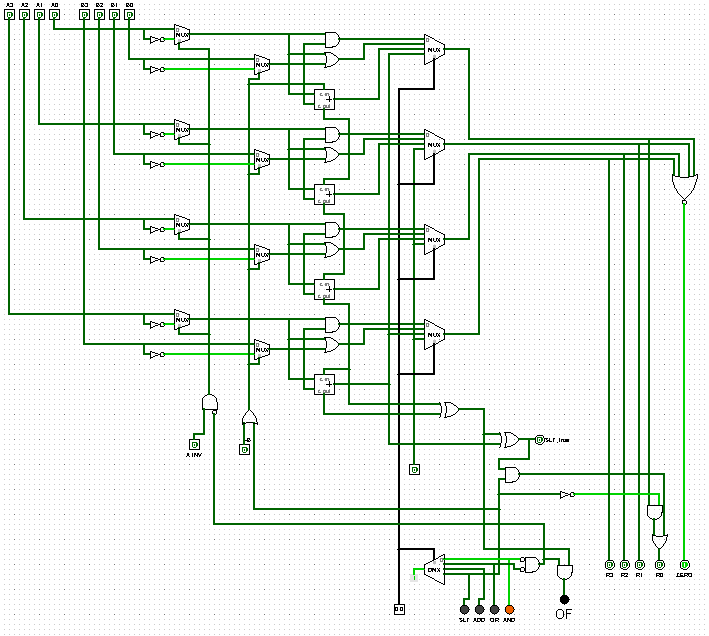
\includegraphics[width=1\textwidth]{media/ula}
    \caption{Interface da ULA de 4 bits. Fonte: Autor}
    \label{fig:ula_interface}
\end{figure}

\subsubsection{Entradas}

\begin{itemize}
    \item $A$: Operando de 4 bits.
    \item $B$: Operando de 4 bits.
    \item InvertA: Sinal de controle para inverter $A$ (1 bit).
    \item InvertB: Sinal de controle para inverter $B$ (1 bit).
    \item $Sel$: Seletor de operação (2 bits).
\end{itemize}

\begin{figure}[H]
    \centering
    \begin{subfigure}[b]{0.45\textwidth}
        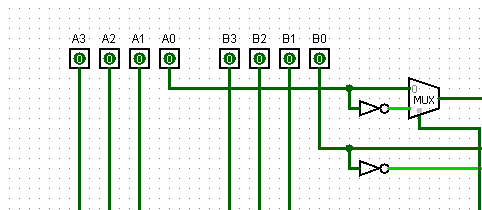
\includegraphics[width=\textwidth]{media/entradas.png}
        \caption{Operandos.}
    \end{subfigure}
    \begin{subfigure}[b]{0.45\textwidth}
        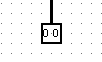
\includegraphics[width=\textwidth]{media/seletor}
        \caption{Seletor de operação.}
    \end{subfigure}
    \begin{subfigure}[b]{0.45\textwidth}
        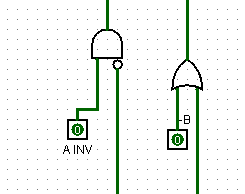
\includegraphics[width=\textwidth]{media/inverters}
        \caption{Inversores dos operandos A e B.}
    \end{subfigure}
    \caption{Entradas Fonte: Autor}
    \label{fig:entradas}
\end{figure}

\subsubsection{Saídas}
\begin{itemize}
    \item $Result$: Resultado da operação (4 bits).
    \item Zero: Flag indicando se o resultado é zero (1 bit).
    \item Overflow: Flag indicando ocorrência de overflow (1 bit).
    \item Operation: Led indicando a operação realizada (1 bit).
\end{itemize}

\begin{figure}[H]
    \centering
    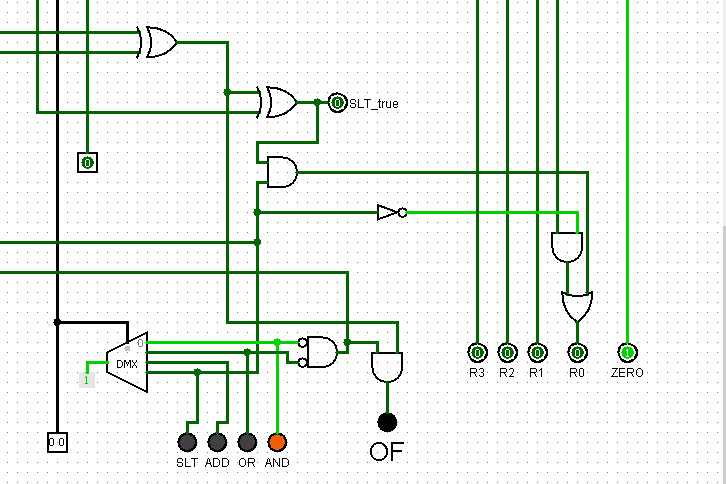
\includegraphics[width=1\textwidth]{media/saidas}
    \caption{Saídas da ULA. Fonte: Autor}
    \label{fig:saidas}
\end{figure}


\subsection{Lógica de Detecção de Overflow}

A detecção de overflow foi implementada utilizando a abordagem baseada nos \textit{carries} do bit mais significativo.
A comparação entre o carry de entrada e o carry de saída do bit mais significativo do somador permite identificar corretamente as condições de overflow para operações de soma e subtração, conforme descrito na seção de fundamentação teórica.

\begin{align*}
    \mathrm{Overflow} &= C_{in,msb} \oplus C_{out,msb}
\end{align*}

A flag \texttt{Overflow} é habilitada apenas para ADD ,SUB e SLT, permanecendo em nível lógico baixo para todas as operações lógicas.

\section{Resultados}

Foram realizados quatro casos de teste representativos, cobrindo overflow positivo, overflow negativo, operação sem overflow e operação lógica.

\subsection{Caso 1: Overflow Positivo (ADD)}

\[
    7 + 1 = -8
\]

O resultado correto seria $8$, que excede o valor máximo representável ($7$). O sinal de overflow foi corretamente ativado.

\begin{figure}[H]
    \centering
    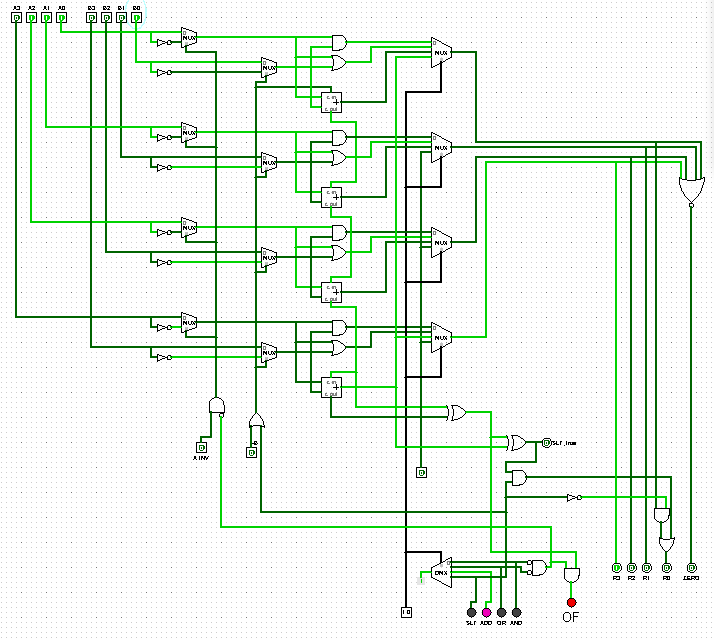
\includegraphics[width=1\textwidth]{media/case1}
    \caption{Caso 1: Overflow Positivo. Fonte: Autor}
    \label{fig:Case1}
\end{figure}

\subsection{Caso 2: Overflow Negativo (ADD)}

\[
    -7 - 2 = 7
\]

O resultado correto seria $-(9)$, abaixo do valor mínimo representável ($-8$). O sinal de overflow foi corretamente ativado.

\begin{figure}[H]
    \centering
    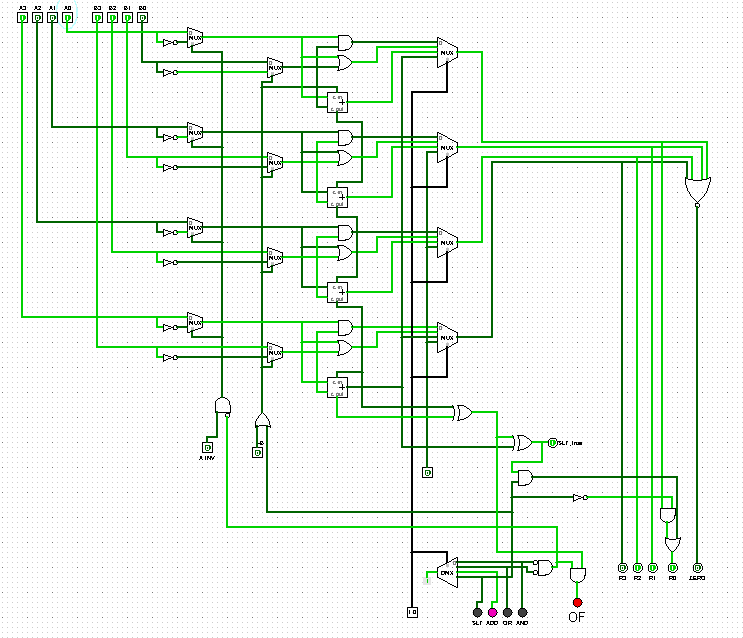
\includegraphics[width=1\textwidth]{media/case2}
    \caption{Caso 2: Overflow Negativo. Fonte: Autor}
    \label{fig:Case2}
\end{figure}

\subsection{Caso 3: Soma Sem Overflow}

\[
    1 + 5 = 6
\]

O resultado está dentro da faixa representável. Overflow não foi ativado.

\begin{figure}[H]
    \centering
    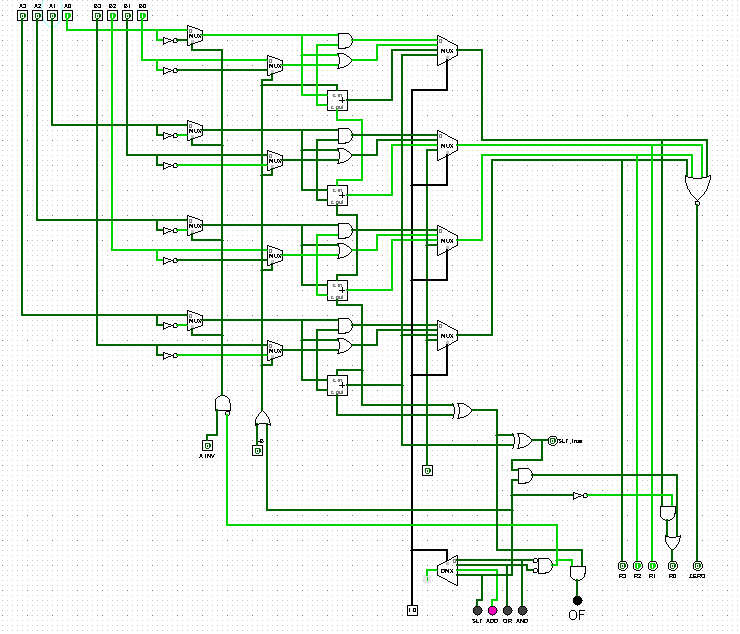
\includegraphics[width=1\textwidth]{media/case3}
    \caption{Caso 3: Soma Sem Overflow. Fonte: Autor}
    \label{fig:Case3}
\end{figure}

\subsection{Caso 4: Set On Less Than (SLT)}

A operação SLT compara $A$ e $B$ e define o resultado como 1 se $A < B$, ou 0 caso contrário. Ela é implementada por meio da subtração $A - B$ e análise do resultado. O overflow é relevante para SLT, pois um resultado incorreto devido a overflow pode levar a uma comparação errada. 
No caso testado, $A = -2$ e $B = 7$, portanto $A < B$ é verdadeiro, e o resultado esperado é 1. A operação $-2 - 7$ resulta em $-9$, que é menor que zero, confirmando a condição de SLT. Entretanto o sinal de overflow é ativado, pois o resultado é não é representável em 4 bits. 
Apesar disso, a lógica de SLT deve considerar o resultado da subtração e não apenas o overflow, garantindo que o resultado final seja correto (1) mesmo com overflow, mostrado na figura \ref{fig:Case4} pelo LED \textbf{$SLT_TRUE$}.
Esse resultado é obtido pela operação: 
\[
    SLT = OVERFLOW \oplus Result_{msb}
\]

\begin{figure}[H]
    \centering
    \includegraphics[width=1\textwidth]{media/slt}
    \includegraphics[width=1\textwidth]{media/slt2}
    \caption{Caso 4: Set On Less Than. Fonte: Autor}
    \label{fig:Case4}
\end{figure}


\subsection{Resumo dos Resultados}

\begin{table}[H]
\centering
\caption{Resumo dos casos de teste}
\label{tab:resultados}
\begin{tabular}{clccc}
\toprule
\textbf{Caso} & \textbf{Operação} & \textbf{Resultado Obtido} &
\textbf{Overflow} & \textbf{Detectado Corretamente?} \\
\midrule
1 & $7 + 1$ & $-8$ & Sim & Sim \\
2 & $-7 - 2$ & $7$ & Sim & Sim \\
3 & $1 + 5$ & $6$ & Não & Sim \\
4 & $SLT(-2, 7)$ & $1$ & Sim & Sim \\
\bottomrule
\end{tabular}
\end{table}

\section{Discussão}

Os resultados demonstram que o mecanismo implementado identifica corretamente situações de overflow em operações de soma, subtração e SLT, sem gerar falsos positivos em operações lógicas.

Vale reforçar que a operação SUB e SLT é implementada por complementação de $B$ seguida de soma, reutilizando o caminho de dados do somador. Isso exige atenção na derivação da condição de overflow para subtração, uma vez que o operando $B$
efetivo é $\overline{B}+1$ e não $B$.

\section{Conclusão}

Neste trabalho foi implementada uma ULA de 4 bits baseada na arquitetura MIPS, suportando as operações AND, NAND, OR, NOR, ADD, SUB e SLT. A lógica de detecção de overflow foi desenvolvida com base na análise dos carries do bit mais significativo do somador, permitindo identificar corretamente situações de estouro aritmético durante operações de soma e subtração.

Os resultados obtidos confirmam o correto funcionamento da implementação: overflow é detectado nos casos de estouro aritmético e suprimido nas demais operações. O projeto permitiu consolidar conceitos fundamentais de arquitetura de computadores, representação numérica em complemento de dois e lógica digital.

\bibliographystyle{IEEEtran}
\bibliography{refs}

\end{document}